\documentclass[a4paper,10pt]{article}

\usepackage[utf8]{inputenc}
\usepackage[english]{babel}
%\usepackage[T1]{fontenc}
\usepackage{graphicx}
\usepackage{wrapfig}
\usepackage{amsmath, amssymb}
%\usepackage{listings}

\begin{document}

\author{Valentin Rosenberg, Zacharias Knudsen}
\date{\today}

\section{Clustering}

\subsection{1}
We will find clusters of a subset of our dataset, as the dataset is meant for regression, many attributes have little or no correlation. We want to examine if there are clusters in the following social and economic attributes:

\begin{verbatim}
['racePctHisp' 'racePctWhite' 'medIncome' 'NumStreet' 'NumImmig' 'PctEmploy'
 'PctPopUnderPov' 'pctUrban']
[[ 0.48042042 -0.35576298 -0.04328459  0.75985761  0.49457753  0.16152224
  -0.04523144  0.68097445]
 [-0.45230355  0.63253709  0.44134997 -0.22663569 -0.27521791  0.18842259
  -0.55648811 -0.11868661]
 [ 0.47569075 -0.74422888 -0.93382755 -0.06608307 -0.21582393 -0.93636532
   1.31695306 -1.06448817]]
\end{verbatim}

\begin{figure}[h]
\centering
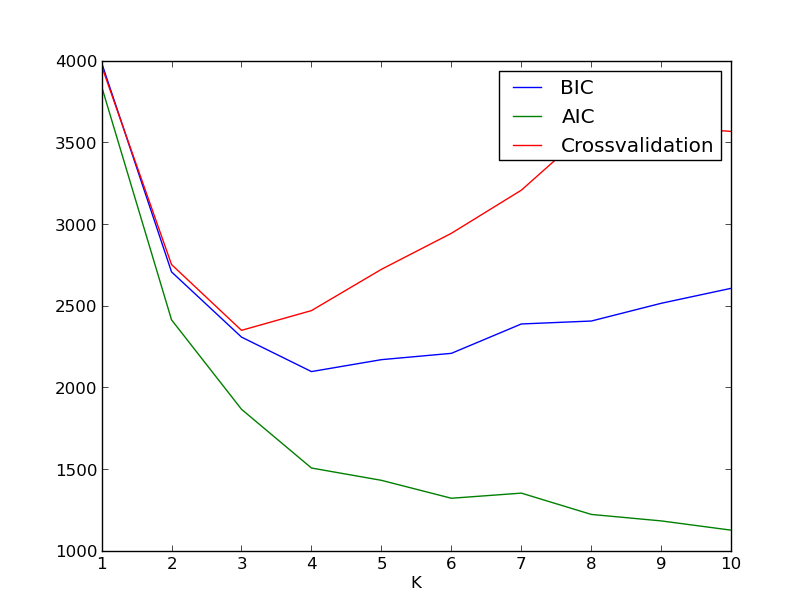
\includegraphics[h, width=0.8\textwidth]{figure_1}
\end{figure}


\end{figure}




\end{document}
